% Instructions to modify this document:
% * Remember to ALWAYS execute a git pull BEFORE any commit you make
% * Use the \ToDo{...} command to remark tasks which still need to be done
% * Use the \input{file.tex} command to split the document into several parts
% * Do not change the current LaTeX coding style to yours

% To convert .dia diagrams into PDF:
% 1) Create the diagram with dia (or any other tool)
% 2) Export it as .eps
% 3) use epstopdf to convert to PDF


\documentclass[a4paper,12pt]{article}

\usepackage[utf8]{inputenc}
\usepackage{amsmath,graphicx}
\usepackage{bm}
\usepackage{amssymb}
\usepackage{algorithm}
\usepackage{algpseudocode}
\usepackage{subfigure}
\usepackage{ifpdf}
\usepackage{url}
\usepackage{color}
\usepackage[hidelinks]{hyperref}
\usepackage{comment}
\usepackage{float} % To put figures in their exact place with \begin{figure}[H]

% Definitions and commands
\def \np{\vskip 0.25 cm}
\def \ap{\vskip 0.15 cm}

\newcommand{\ToDo}[1]{\textcolor{magenta}{\textbf{[ToDo]} \textbf{#1}}}


\begin{document}


\begin{titlepage}

\begin{center}
\vspace*{-1in}

%Universitat Oberta de Catalunya\\
\vspace*{0.6in}
\begin{Large}
\textbf{The IPOL Demo System} \\
\end{Large}
\vspace*{0.6in}
\rule{80mm}{0.1mm}\\
\vspace*{0.1in}
\end{center}

\end{titlepage}

%\maketitle
\newpage

\tableofcontents
\newpage
\listoffigures
\newpage


% The Blobs module
\section{The Blobs module}

Note: to avoid confusion, we refer the modules of the IPOL system as ``ipol modules'' and Python modules (files containing Python code) as ``Python modules''.

\subsection{Introduction}
Each demo of IPOL offers the user a set of defaults blobs. Thus, the users are not forced to supply their own files for the executions of the algorithms. These defaults blobs can be tagged and linked to differents demos.

\subsection{Composition}
The blobs module is composed of several Python modules. It is composed of the same technical stack as the rest of the rest of the IPOL modules: written in Python, using a web server, a database, and using templates for generating HTML responses for webservices destinated to humans.

\subsubsection{Main Python module}
The main module is called by ``start.sh'', the script called by the control terminal to get modules running on different servers over ssh. It consist of setting up some variables used by cherrypy, as well as mounting the blobs class at the root of the used server.

\subsubsection{Error Python module}
This module describes the errors issued by the Blobs IPOL module and adds color to the error messages printed in the terminal.

\subsubsection{Database and database Python module}
The first and most important design constraint of the Blobs IPOL module was that data shouldn't be duplicated. All blobs referenced by multiple demos should exist in only one directory. This is addressed by establishment of one relational database, referencing the demos, the blobs, and the relationship between them. This database also permits to tag some text on blobs, as well as organize them in named sets. In the big picture, the database Python module a implement a simple CRUD\footnote{Acronym for Create, Read, Update, Delete. These operations allows the total manipulation and the persistancy of data inside a data structure.} interface for manipulating the database. Blobs can be managed individually, and upon the deletion of a demo, the blobs related to this demo will be deleted from disk if and only if they were uniquely linked to this demo. Blobs are referenced via their hashes, making it easy to verify if a blob is already in the database, even under another filename. \\

\begin{figure}[h]
\centering
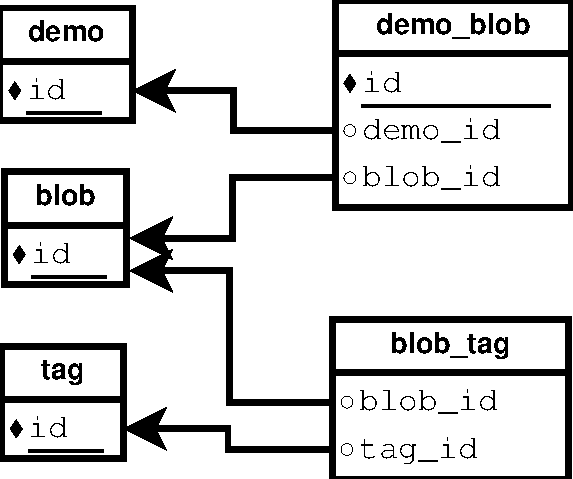
\includegraphics[scale=0.75]{blobs/images/blobs_database.pdf}
\caption{The database architecture of the blobs module} 
\label{fig:blobs_database}
\end{figure}


In the figure~\ref{fig:blobs_database}, id fields are the primary keys (it is worth noting that the primary key of a blob\_tag entry is the combination of the foreign keys it contains), the other fields are foreign keys, and the arrows indicate which primary keys are referenced by which foreign keys.
Three tables, demo, blob and tag, contains the information about referenced demos, blobs, and tags relating to blobs. Two junction tables link this information together, referencing the blobs standards to a demo, and the tags owned by each blobs.

\paragraph{The database Python module\\}
This module offers an interface for accessing the database. One object of the class Database should be instanciated for each operation modifying it. Even if it has function for connecting and closing, they should not be used as such, for flow control issues (for example, an exception leaving a connection open). A very simple abstraction, the DatabaseConnection class is present in the blobs Python module for it, and allow safe connection to the database, ensuring they will always be closed no matter what.

Otherwise, this Python module offer us a wide variety of simple methods for interacting with the database, or obtaining metrics of it, such as the total number of blobs. They generally return the information asked if such case apply. For the format of the responses and the different function, we refer the reader to the code of the module itself. It is worth noting that one webservice, delete\_blob\_from\_demo, recompute the positions of the blobs in a set in which a blob was deleted. If this function is accessed concurrently by multiple threads (the most likely case is if a webservice calling this function is accessed several times in a very short span), the blobs can end up with miscalculated positions. Non-concurrential access should be enforced by locking the scope where this webservice is called. Such a lock is used in the delete\_blob\_ws webservice in the blobs Python module.

\subsubsection{Blobs module}
The blobs Python module is the core of this. It implement three classes, DatabaseConnection as referenced earlier in the present documentation, and MyFieldStorage, for intermediate storage of the uploaded blobs in the /tmp/ directory, and Blobs as an encapsulation of the webservices and the data they use. It also has some utilitary function.

The Blobs class implements all the webservices constituting this module, both those transmitting JSON to other modules, and those generating HTML via templates for humans. An instance of the Blobs class should possess information about the storage of blobs and the networking parameters cherrypy use, such as a port number. A cherrypy configuration file, named ``blobs.conf'' contains the informations one might need to change to run the module on another server, without changing the code, such as the directories where the blobs can be found, the port used by the cherrypy engine, or the path to the database.

The webservices of the module access the database via instanciations of Database objects managed by the DatabaseConnection class. Some read information, and some modify the database by adding or removing information. For handling a webservice automatically and charging his JSON response as a Python object, the utilitary function use\_web\_service is used.

Logging is utilized as a mean to retrieve the errors occuring in the system. The logger implemented in the blobs Python module handle all the errors of the module. It is passed to each Database object instanciation.

Here is a list of all the webservices implemented by the blobs module :

\begin{itemize}
\item default : The service invoked when asked for non-existing service.
\item index : web page at the root of where the module is mounted in cherrypy.
\item blob : web page used to upload one blob to one demo.
\item archive : Used to upload one zip file of compressed blobs to one demo.
\item add\_blob\_ws : service checking that the given blobs do not exist in the database. If this is the case, add it.
\item add\_blob : implement the add\_blob page.
\item demos\_ws : return the list of demos from the database.
\item get\_template\_demos\_ws : return the list of template demos from the database
\item demos : web page used to add a demo to the database.
\item set\_template\_ws : webservice used to change the template used by a demo.
\item use\_template : web page used to change the template used by a demo.
\item add\_demo\_ws : web service used to add a demo to the database.
\item add\_demo : web page used to add a demo to the database.
\item add\_from\_archive : webservice used to upload a zip file of compressed blobs to one demo.
\item add\_tag\_to\_blob\_ws : webservice used to add a tag to a blob.
\item op\_add\_tag\_to\_blob : web page used to add a tag to a blob.
\item remove\_tag\_to\_blob\_ws : webservice used to remove a tag from a blob.
\item op\_remove\_tag\_to\_blob : web page used to remove a tag from a blob.
\item op\_remove\_blob\_from\_demo : web page used to remove a blob from a demo.
\item get\_blobs\_from\_template\_ws : webservice used to get the list of blobs from templated demo.
\item get\_blobs\_of\_demo\_by\_name\_ws : webservice returning a list of the hashes of the blobs owned by given demo name.
\item get\_blobs\_of\_demo\_ws : same as the precedent, but with the demo id.
\item get\_blobs\_of\_demo : web page used to display blobs owned by a given demo.
\item edit\_blob : web page showing the thumbnail of a demo with the possibility to add or remove tags.
\item get\_blob\_ws : webservice returning information about a blob from its id.
\item get\_tags\_ws : webservice returning tags of a blob from its id.
\item op\_remove\_demo\_ws : webservice removing a demo from its id.
\item op\_remove\_demo : web page used for removing a demo.
\item ping : used by the terminal for checking module status.
\item shutdown : used by the terminal for turning off the module at distance.
  
\end{itemize}


% The Archive module
\section{The Archive module}

\subsection{Introduction}
\label{sec:archive_introduction}

%\paragraph{Introduction} \hspace{0pt} \\
The archive module is a standalone application destinated to communicate with other modules using webservices. It is designed to implement a stable, simple and scalable system for archiving all experiments done with IPOL.

\paragraph{Technologies used} \hspace{0pt} \\
The archive module is written in Python, is using the cherrypy framework for webservices, the mako template library for webpage rendering, the Python Image Library for thumbnails creations, and the python-magic library available on pip (not to be mistaken with python-magic5 which is the one available on default ubuntu's APT repositories). The module communicate using JSON, both in input and output. The database engine used is SQLite.

\subsection{Architecture}

\paragraph{Module composition} \hspace{0pt} \\
The module is composed of very few files, the code itself in ``module.py'', a cherrypy configuration file ``archive.conf'', two mako HTML templates, and a database. It will also need 4 directories, respectively for storing blobs, thumbnails, the database and logs.

\paragraph{Module architecture} \hspace{0pt} \\
The module is composed of a class, Archive, encapsulating the datas needed to function. The services offered by the module are all methods of this class. The cherrypy framework provide the abstraction for making available the methods as webservices. \\
Upon starting the module, the cherrypy engine is launched, an object of the Archive class is created, and the cherrypy configuration is loaded from ``archive.conf''. If they don't exists, both the database and the directories needed for the storage of blobs, logs, the database and thumbnails will be created, provided that the user launching the module has the necessary rights. Otherwise, the module will not start. These directories are indicated in the cherrypy configuration for maximum configurability, if they are missing from it, the module will not start. \\
The webservices communicate with the server via arguments given through URL, as unicode strings directly passed to the methods. \\
The services all connect to the database in a thread-safe way, instanciating its own connection when called, commiting when done if there is modifications, or rollbacking if there is an error, and closing the connection. \\
There is a logger initialised with the Archive object, writing errors in ``error.log'' in the logs directory given in the configuration file.

\subsection{Database design}

The database contains 3 tables : experiments, blobs, and correspondence.\\
Each experiments, and each blobs are defined individually, and linked to each-others in the correspondence table, assuring a many-to-many connection. It is worth noting that the database doesn't save duplicates of the same blob. \\

\begin{tabular}{|l|c|r|}
  \hline
  experiments & blobs & correspondence \\
  \hline
  id & id & id \\
  id\_demo & hash & id\_experiment \\
  params & type & id\_blob \\
  timestamp & format & name \\
  \hline
\end{tabular} \\

\paragraph{Experiments table} \hspace{0pt} \\
The experiments table is defined as such : the id field, that store the unique id of the experiment ; the id\_demo field, that store the id of the IPOL demo used for the experiment ; the params field, which is a JSON string whose format vary from demo to demo ; and finally the timestamp field.

\paragraph{Blobs table} \hspace{0pt} \\
The blobs table is defined as such : the id field, that store the unique id of the blob ; the hash field, that store the hash of the blob computed with sha1, the type field, that store the extension of the blob (exemple ``jpeg'' or ``png''), and the format field, that store the media format of the blob : it is a string, either ``audio'', ``video'' or ``image''. \\
The physical location of a blob is ``blob\_dir defined in configuration file'' + ``hash of the blob'' + ``.'' + ``type of the blob''.

\paragraph{Correspondence table} \hspace{0pt} \\
The correspondence table is defined as such : the id field ; the id of the experiment and the id of the blob that is linked to said experiment, and the name field, which indicate the role of the blob in the experiment (example : ``input'' or ``denoised''). A foreign key constraint allowing cascade delete is put on the field id\_experiment, referencing the id of an entry in the experiment table, for automatic data deletion.

\subsection{Services}

\paragraph{Adding an experiment to the archive} \hspace{0pt} \\
The method ``add\_experiment'' take in entry the id of the demo used ; a JSON string of the format : 

\begin{tabbing}
tabs \= tabs \kill
\{ \\
\>url\_blob : name\}, \\
\> ... \\
\} \\
\end{tabbing}

containing a description of each blobs used by and produced by the experiment, with their temporary URLs and names ; and a JSON string describing the parameters of the demo used for the experiment. It will add an experiment to the database by creating a new entry in the experiment table. If the blobs used by and produced by the experiment aren't already in the database, it will copy them in the directory given in the configuration file, and, for the images, create a thumbnail. It will return a json string containing the status of the operation, OK uf it succeeded, KO if there was an error and the operation wasn't performed, as such :

\begin{tabbing}
tabs \= tabs \kill
\{ \\
\>status : OK/KO\}, \\
\} \\
\end{tabbing}

If status is KO, a log describing the error will be written.

\paragraph{Deleting an experiment from the archive} \hspace{0pt} \\
When removing an experiment from the database via the method ``delete\_experiment'', every blobs linked to this experiment and only to this experiment are removed. After that, all the entries in the correspondence table referencing this experiment are removed automatically due to a foreign key constraint. It return a json response containing the status of the operation of the same format as the return of the method ``add\_experiment''.

\paragraph{Deleting a blob from the archive} \hspace{0pt} \\
Due to a many-to-many link between blobs and experiments in the database, a blob has a lot of dependencies : it has of course the experiments using this blobs, but also the blobs linked to these experiments. For deleting a blob from the archive, the precedent service is called on each experiment the blob is part of, assuring that no orphans datas stay in the database (for exemple, experiments linked to removed blobs or blobs linked to removed experiments). The method implementing this service is ``delete\_blob\_w\_deps''. It return a json response containing the status of the operation of the same format as the return of the method ``add\_experiment''.

\paragraph{Getting datas from an archive page} \hspace{0pt} \\
The method ``page'' return in a JSON response, for a given page of a given demo, all the datas of the experiments that should be displayed on this page. Twelve experiments are displayed by page. For rendering the archive page in the browser, the JSON response should be parsed and interpreted in a dedicated template furnished by the front-end of another module. The JSON response is formatted this way : 
\begin{tabbing}
tabs \= tabs \= tabs \= tabs \= tabs \= tabs \kill
\{ \\
\> status :  OK/KO, \\
\> experiments : [ \\
\> \> \{ \\
\> \> \> date : timestamp\_example, \\ 
\> \> \> files : [ \\
\> \> \> \>  \{ \\
\> \> \> \> \> url : url\_example, \\
\> \> \> \> \> id : id\_example, \\
\> \> \> \> \> name : name\_example, \\
\> \> \> \> \> url\_thumb : url\_thumbnail\_example \\
\> \> \> \> \} \\
\> \> \> ... ], \\
\> \> \> id : id\_example, \\
\> \> \> parameters = \{parameters\_example...\} \\
\> ... ], \\
\> id\_demo : id\_demo\_example, \\
\> nb\_pages : nb\_pages\_example \\
\} \\
\end{tabbing} 

\paragraph{User interface for removing blobs/experiments} \hspace{0pt} \\
The only user interface furnished by the archive module is for removing blobs or experiment in a convenient manner. It use the json response of the precedent service and render the ``archive\_admin\_tmp.html'' template displaying a page of archive for given demo, allowing the deletion of both blobs and experiments by simply linking to two other services calling deletion methods and updating the template. In case of error, for example when invalid datas are given through URL, ``error.html'' is rendered.

\paragraph{Shutdown} \hspace{0pt} \\
The method ``Shutdown'' shutdown the archive application when called. It return a json response containing the status of the operation.

\paragraph{Other services}
Other services features the method ``ping'', simply for checking if the module is up, and the method ``stats'', formatted this way :
\begin{tabbing}
tabs \= tabs \kill
\{ \\
\> status : OK/KO, \\
\> nb\_experiments : x, \\
\> nb\_blobs : y \\
\} \\
\end{tabbing}




\end{document}
% End of document

